\documentclass{article}

\usepackage[printqrbox=false,printhint=false,printanswer=true,printmarkingguide=false,printdraftpaper=false]{unswalgos}

\usepackage{tikz}
\usetikzlibrary{patterns}
\usetikzlibrary{shapes,fit}
\usepackage{tkz-fct}
\usepackage{wrapfig}
\usepackage{subfig}

\usepackage{mathtools}
\usepackage{amssymb}
\usepackage{booktabs,multicol,multirow}
\usepackage{wasysym}
\usepackage{tcolorbox}

\DeclareMathOperator*{\argmax}{arg\,max}
\DeclareMathOperator*{\argmin}{arg\,min}
\DeclareMathOperator{\NAND}{NAND}
\DeclareMathOperator{\AND}{AND}
\DeclareMathOperator{\OR}{OR}
\DeclareMathOperator{\NOT}{NOT}

\usepackage{xspace}

\fancyfoot[L]{\leftmark}
\fancyfoot[R]{\rightmark}

% This enables new paragraphs without indentation
\usepackage[parfill]{parskip}

\usepackage{graphicx}
\usepackage{float}
\usepackage{subfigure}

\newcommand{\sem}{22T2}
\newcommand{\semester}{Term 2, 2022}
\SubjectNo{COMP3151}
\newcommand{\taskname}{Assignment 0}
\Institution{Jinghan Wang, z5286124} % Replace this with your name and zID


\begin{document}
\Large\textbf{Task}\\\\
\normalsize
Consider the following algorithm presented in Ben-Ari's notation.
\begin{figure}[H]
    \centering 
    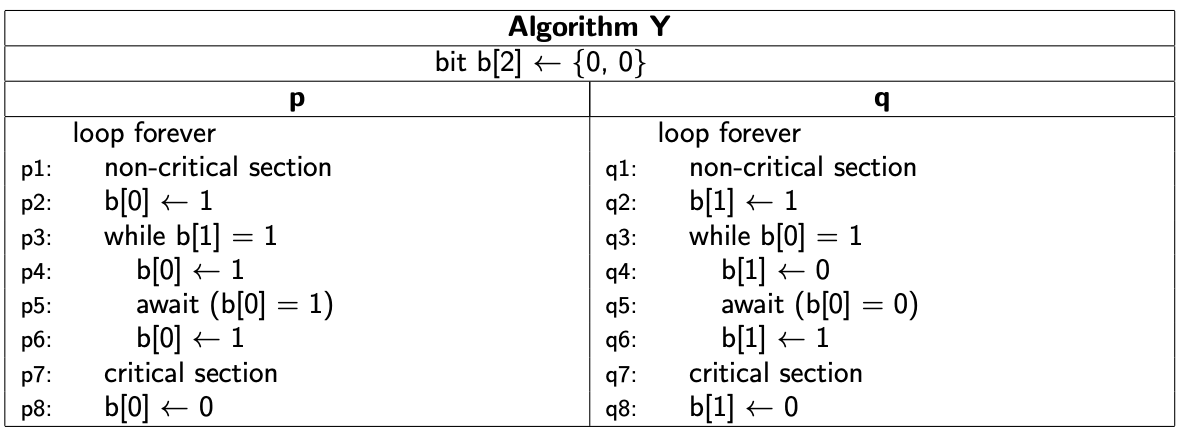
\includegraphics[width=0.95\textwidth]{DV_demand}
\end{figure}


\begin{Question}
\textbf{[40 marks]} Use Spin to check whether Algorithm $Y$ is a solution to the critical section problem. Address all four desiderata from the lectures (mutual exclusion, eventual entry, absence of deadlock, absence of unnecessary delay).

\begin{answer}
    Answer:\\
\end{answer}
\end{Question}




\begin{Question}
\textbf{[40 marks]} Encode Algorithm $Y$ as a parallel composition of two transition diagrams. Define an assertion network $Q$ such that the assertions at the locations representing the critical sections express mutual exclusion. Prove that $Q$ is inductive. (It is ok to focus on the processes after the initialisation of b. It is not ok to make the assertions at the entry locations unreasonably strong.)
\begin{answer}
    Answer:\\
\end{answer}
\end{Question}




\begin{Question}
\textbf{[20 marks]} Identify any superfluous statements in the algorithm. That is, can any statements be replaced by $skip$ without changing the behaviour of Algorithm $Y$? Justify your answers, preferrably using your transition diagram and assertion network.
\begin{answer}
    Answer:\\
\end{answer}
\end{Question}




\end{document}